\documentclass[letterpaper]{article}
\usepackage{aaai}

\usepackage{times}
\usepackage{helvet}
\usepackage{courier}

\usepackage{graphicx}

\pdfinfo{
/Title (YARP)
/Subject (YARP)
/Author (IIT)}

\title{YARP, a Thin Middleware for (Humanoid) Robots}
\author{Paul Fitzpatrick \and Giorgio Metta \and Lorenzo Natale \\
Italian Institute of Technology \\
Via Morego, 30 \\16163 Genova, Italy}
\setcounter{secnumdepth}{0}

\begin{document} 
\maketitle
\begin{abstract}
\begin{quote}

YARP stands for ``Yet Another Robot Platform.''  It is a robot
middleware that began life in 2000 as a thin layer over the QNX
real-time operating system to adapt it for use by humanoid robots.  It
is now used on all kinds of operating systems and robots around the
world.  YARP's communication model lies at a sweet spot that combines
efficiency, flexibility, and ease of use.

\end{quote}
\end{abstract}

\noindent 

YARP is plumbing for robot software.  YARP supports building a robot
control system as a collection of programs communicating in a
peer-to-peer way, with an open-ended family of connection types (tcp, udp,
multicast, local, MPI, mjpg-over-http, XML/RPC, tcpros, ...) that can
be swapped in and out to match your needs.  It also supports similarly
flexible interfacing with hardware devices. Our strategic goal is to
increase the longevity of robot software projects
\cite{fitzpatrick08towards}.

YARP was, in its early days, shaped by the problem of keeping research
going despite constant flux in our robot platforms (hence the name).
Long experience with incompatible ``architectures,'' ``frameworks,'' 
and ``middleware'' (which we like to call collectively ``muddleware'')
has taught us to make YARP a {\it reluctant} middleware, 
with no desire or expectation to be in control of your system.
YARP is not an operating system, or a package manager.  

\begin{figure}
\centerline{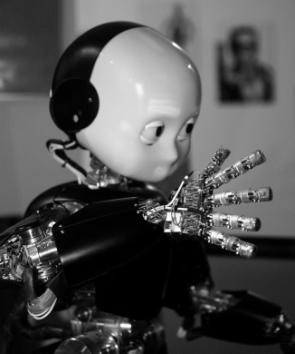
\includegraphics[width=5cm]{icub.jpg}}
\caption{YARP is used on
complex humanoids such as the iCub (pictured here),
on embedded systems, and everything in between.
} 
\end{figure}

\section{Robot evolution}

Robot technology and information technology in general is a
fast-moving target.  With YARP, we've taken the following steps to
help our users lead:

\begin{itemize}

\item YARP's implementations of different connection types, called
carriers, are designed as replaceable plugins.  New network types can
be accommodated through new carriers.  New versions of a particular
carrier can be evolved over time, and co-exist with older versions,
without sudden breaks of backwards compatibility.  Interoperation
with other middleware or data sources/sinks can be systematically
added.

\item YARP strongly encourages users to access devices via sets of
interfaces that allow for similar evolution.

\item We rely on carefully chosen dependencies, namely ACE and CMake,
to help us keep up with churn in operating system releases, IDEs, and
other parts of our users' toolchains.

\end{itemize}

\section{A potted history of YARP}

YARP was born in 2000 on an early humanoid robot (called Kismet)
controlled by a set of Motorola 68332 processors, an Apple Mac, and a
loose network of PCs running QNX, Linux, and Microsoft Windows
\cite{metta06yarp}.  Communication on this robot was a cocktail
mixture of dual-port RAM polling, QNX message passing, CORBA, and raw
sockets.

YARP worked very well on QNX, and decently on Linux.  For Microsoft
Windows, Macs, and other platforms an important development in YARP's
history was to take on a dependency on the ACE library [ref].  This
happened around 2003, with the immediate goal of simplifying the
addition of multicast support.  ACE has proven its worth to us many
times over for cross-platform networking, although we needed
to carefully keep any reference to ACE out of public header files
in order to avoid inheriting some of its less desirable properties
(a somewhat unstable API, and constraints on header file inclusion
order).

When YARP grew an image processing library, care was taken to make the
data structures compatible with the IPL library (a non-free image
processing library from Intel).  IPL became the seed for OpenCV, which
also remained compatible with IPL. YARP has therefore somewhat
accidentally played nicely with OpenCV, which has grown to be a very
popular library, from the start.

YARP developers were early and enthusiastic adopters of CMake
\cite{fitzpatrick10cmaking}.  In 2006, we happily dumped
earlier custom build scripts in favor of CMake project descriptions,
and never looked back.  CMake was this missing piece for having a
truly comfortable cross-platform experience.

About the same time, we started using SWIG [ref] to support languages
other than C++.

Use of CMake and SWIG has become common in open source libraries.
The help users exploit software on many operating systems and 
languages.  By keeping YARP as ``just a library,'' there is no
obstacle to doing the same with YARP.  But since YARP facilitates
intercommunication, this has the powerful effect of allowing 
programs written in all these environments to communicate with
each other, and easily.

\section{Data liberation}

Google has a subproject to make sure that it is easy for users to copy
all their data from a service in usable form, and migrate to a
non-Google service: the ``data liberation front.''  Having such 
a project is a way to keep themselves honest, and avoid the 
temptation of using control of data as a way to lock people in to
using their services.

For YARP, we try to make it easy to users to redirect data streams to
non-YARP based programs.  This lowers the cost of ``boundary
problems'' such as hooking up an unsupported device, computer,
network, or collaboration between people from different planets
(e.g. computer science versus developmental psychology versus
neuroscience).

The protocol used for a YARP connection is decided at connection-time.
The initiator of the connection is free to choose from a wide set of
protocols, and so can optimize for simplicity (using a plain text
protocol), speed (udp), scalability (multicast), etc.

A YARP protocol need not be specific to YARP.  For example, YARP
supports mjpeg-over-http.  This means that a YARP image source can be
viewed directly from a browser without bridging, or a YARP image sink
can receive data directly from a jpeg-streaming IP camera without
bridging.  YARP also supports XML/RPC, so can connect to certain
websites (or act as a webserver).

YARP connections can be initiated by either the "sender" or
"receiver", since the logical flow of data can be freely reversed.
This is important for supporting a wide range of protocols, which may
be "pull" or "push" in nature.  It also makes connecting to YARP
programs without using the YARP libraries even easier.  With other
middleware, you get stuck having to make a server for at least one of
the directions of data flow.

A YARP network is designed to be usable without YARP.  Examples of
making YARP connections without using the YARP library are available
in C and Python.


\section{The TELNET test}

The TELNET test is this: can a user monitor and insert traffic on a
YARP network using just a telnet client (``telnet ip.address
port\_number'')?  In other words, without any use of YARP libraries or
programs?  This test has evolved out of past frustration with other
middleware, where simply passing a few numbers to a collaborator's
program can require jumping through a dozen hoops.  We try to follow
the ``golden rule,'' by making it really easy for others to send a few
numbers to a YARP-based program without having to dig through protocol
specifications, or link against our libraries, or use our build
machinery~-- all of which can be much more expensive in developer time
than one might think, given the variety of languages, operating
systems, development environments, and versions-of-everything in use.

Some keys to acing the TELNET test:

\begin{itemize}

\item TCP connections should be supported.  
  This is true of most middleware operating on regular
  networks. Some just support UDP, so this test doesn't
  make sense for them.

\item The basic communication model shouldn't stray too far from the
  notion of making ``connections'' to a named destination.

\item The direction in which a connection is initiated shouldn't
  determine the direction of data flow.

\item Human readable/writable.

\end{itemize}


\section{Building on YARP}

Others have built on YARP.

\begin{quote}
``Compared to, e.g., CAVIAR and Psyclone, YARP
looks like a fairly standard library~- neither does it
do its own message scheduling nor does it provide
heavy-handed semantics for message definitions or
networking. That may be its very strength.'' \cite{stefansson09yarp}
\end{quote}

\begin{quote}
``YARP was chosen as the communication library with
which all communication protocols were implemented as
one of the goals of the design of the communication stack
was to make it possible to interact with programs that are
developed without using MeRMaID.'' \cite{barbosa09mermaid}
\end{quote}


\section{Known carriers}

\begin{tabular}{|l|p{7cm}|}
\hline
\multicolumn{2}{|c|}{YARP carriers} \\
\hline
tcp & Regular tcp \\
fast\_tcp & Variant that drops flow control \\
udp & UDP \\
http & Basic web interface \\
mcast & Multicast - avoid repeating the same data going
to many clients ``on the wire''  \\
local & local \\
mpi & delegate to MPI (Daniel Krieg) \\
xmlrpc & translate messages into XML/RPC compatible form \\
tcpros & interoperate with ROS publisher/subscribers \\
mjpeg & receive/transmit images in mjpeg-over-http format \\
text & send messages in human readable plain text form \\
shmem & use shared memory \\
\hline
\end{tabular}

Similarly, many devices.


\section{YARP plus/minus}

YARP core libraries and their full dependencies are light.
YARP has for example been used on an embedded system
with 54MB RAM, 28MB Flash.

YARP is portable, serving an interdisciplinary community.

No code generation, no special build system, doesn't try to take over.

Flexible, open model of connections - proving good for evolution and interoperation.

Passes the ``telnet test''.

Negatives:

Native implementation exists only in C++.  

Diverse OS support limits growth of library, since any
new dependency is very costly.

Lack of IDL / code generation can lead to some tedium
implementing classic RPC-style code.


\section{Scrap}


Ideally, users of robot middleware would cleanly separate out their
algorithmic work from the messy plumbing associated with particular
robot setups.  But in practice, it is quite uncommon for users to do
this, and it causes problems later as setups change or they try to
collaborate with others.  YARP tries to save users from themselves
by reducing the problems it causes.  Specifically:

\begin{itemize}

\item No constraint on future OS and IDE.

\item LPGL licensing.  Not complete freedom, but not bad.

\item A collaborator need not be using YARP.  It is practical to
communicate with a YARP-using program without using YARP.

\item If a collaborator is willing to link extra libraries in their
programs, they can use YARP without disturbing their existing
middleware.

\end{itemize}

It is easy to interoperate with YARP-using programs
without yourself necessarily having to use YARP. 
YARP is written in C++, with a core that uses
no external libraries, not even the standard template libraries, with
the exception of a small portion of ACE for portability (and this
portion can easily be embedded). YARP is free and open.  The
core YARP libraries are released under the LGPLv2.1.


\bibliography{yarp}
\bibliographystyle{aaai}


\end{document}
